\chapter{Marco teórico y contexto tecnológico}
\label{chapter:background}

\section{Marco Teórico}

En este capítulo se introducen los conceptos teóricos sobre los que se asienta el desarrollo de este proyecto. Con el contenido de este capítulo se espera
crear un base de conocimiento sobre la que desarrollar el resto de este documento. Además, se realiza un análisis de las herramientas que se van a emplear para desarrollar el sistema y cómo estas se encuadran en el contexto tecnológico actual.

\section{Sistemas IoT}

Tal y como se introdujo de manera informal en el capítulo anterior, \textit{IoT} se define como un sistema global e inteligente
sistema con conciencia global, transmisión fiable
y procesamiento inteligente de datos %\cite{noauthor_8_2020}.

En este sentido una arquitectura de alto nivel, basada en el conjunto de capas de todos estos objetos interconectados puede verse representada gráficamente en la Figura \ref{fig:IoT_General}.

\begin{figure}[H]
  \centering
  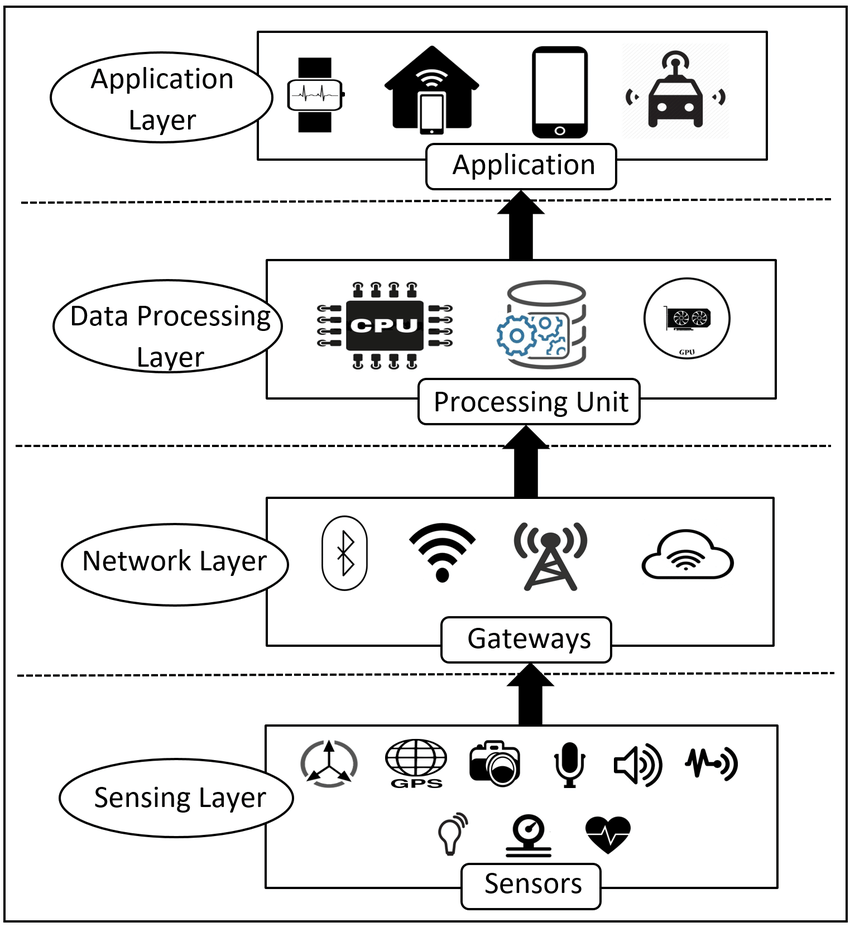
\includegraphics[width=0.7\linewidth]{figures/IoT-Architecture-Layers-and-Components.png}
  \caption{Diagrama general de un sistema IoT}
  \label{fig:IoT_General}
\end{figure}


\section{Contexto tecnológico}

Esta sección recoge la información relativa a las tecnologías y herramientas más relevantes dentro del contexto del desarrollo de este proyecto.

